\chapter{Background}
\label{chapter:background}

This thesis is focused on Hyperledger Fabric. It is a permissioned blockchain project aimed at creating a framework for blockchain solutions. The network and the consensus protocol are the hardest parts of the blockchain to implement and Hyperledger Fabric provides the plug-and-play solution to this problem. The programmer only needs to implement the transaction logic he or she wants and upload it as a chaincode to get a functioning blockchain.

In this chapter, we will illustrate relevant parts of the Hyperledger Fabric, explain concepts necessary for understanding the thesis, and focus on parts of the framework we intend to modify.

Hyperledger Fabric itself is written in Go programming language. There is also an SDK for developing client applications written in NodeJS.
However, knowledge or proficiency with Go or NodeJS is not required for understanding the thesis.

\section{Network}
\label{sec:network}

In this section, we will dissect a basic network architecture. This example is based on the network used in chapter \ref{chapter:evaluation}. The section is based on \cite{fabricdocs:network}

For simplicity, the network has only one channel and two organizations.

\vskip 0.5cm

\begin{figure}[hp]
\begin{center}
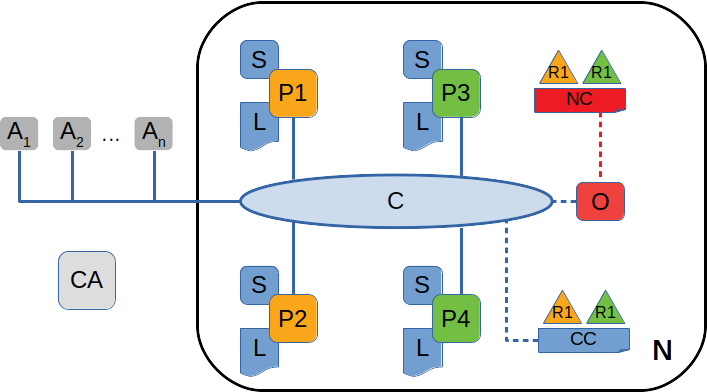
\includegraphics[width=0.95\textwidth]{figures/network}
\end{center}
\caption{Example of a Fabric network}
\label{fig:net}
\end{figure}

The network consists of two organizations $R1$ and $R2$. The network is under control of both R1 and R2 and is governed according to policy rules specified in the network configuration $NC$.

The network has four peers. Peers $P1$ and $P2$ belong to organization $R1$ and peers $P3$ and $P4$ belong to $R2$.

All four peers have joined a channel $C$ and maintain a copy of the channel's ledger $L$ and have a smart contract $S$ installed.

The channel is governed according to a channel policy, defined in channel configuration $CC$ and is controlled by both organizations.

An ordering service $O$ supports the channel and is ordering the channel's transactions into blocks and distributes blocks to the peers. It also serves as an administration point for the network. For administrative purposes, the ordering service uses a system channel, not shown in the diagram. The system channel is mandatory for any network and thus implicit.

Certificate authority $CA$ and applications $A_{1} ... A_{n}$ are not part of the network and in this specific case do not belong to a particular organization. In a general case

Applications are connected to the channel and can use its ledger and smart contract hosted on the peers to generate transactions and submit them to the ordering service. In this case, any application can use any peer to invoke the smart contract but in a general case, an application can only connect to peers from its organization.

Certificate authority issues and confirms certificates that are used to establish which applications or parts of the network belong to which organization. In this case, $CA$ is used by both organizations but in a general case, each organization can host its certificate authority server.

% \newpage

\section{Transaction flow}
\label{sec:flow}
This section describes a transaction flow or a transaction's lifecycle. The section is based on \cite{fabricdocs:flow},  \cite{fabricdocs:peer} and \cite{fabricdocs:orderer}

Fabric's transaction lifecycle consists of three phases
\begin{itemize}
  \item Proposal
  \item Ordering and packaging transactions into blocks
  \item Validation and commit
\end{itemize}

Let's say a client application wants to perform a transaction. It creates a transaction proposal and sends it to all peers whose signature is required, according to channels endorsement policy.
A peer receives the transaction proposal, checks that a client has necessary rights etc and executes it against the current ledger. The execution yields a read-write set. The set contains the keys which are read from and written to during the execution. The read part of the set also contains version value for each key. Versions are used later in the validation phase. The write part of the set contains keys and values that are to be written to commit the transaction to the ledger. The read-write set is then included in the response to the client and signed by the peer. The resulting structure is sent to the client. This concludes the Proposal phase.

When the client has collected all the required endorsements it checks them for consistency, packs them into a transaction envelope and sends the envelope to the ordering service. There can be different implementations of the ordering service, but they all perform the same function. The orderer receives transaction envelopes from different clients and assembles the incoming envelopes into blocks. After a  block is created, the order of transactions within it is fixed. The orderer then distributes the newly created block among the peers of the channel. This concludes the Ordering phase.

When a peer receives a block it goes through all transactions in the exact order they appear in the block. The peer checks signatures of a transaction and makes sure that it complies with the endorsement policy. Read-write sets from different endorsements are also checked for consistency. If a transaction passes all checks, the peer attempts to apply it to the ledger. Before applying a transaction, a ledger consistency check is done. The peer checks versions of the read keys to see if any of the keys were modified after the proposal was endorsed. If ledger state is compatible with the transaction, the transactions write set is applied and the transaction is marked as valid within the block. Invalid transactions are not applied but are marked as invalid and kept for accounting. The block is then appended to the chain and stored. Finally, the peer generates events, signaling to all subscribers which transactions were commited. This concludes the final phase of a transaction's lifecycle.

\section{The structure of a peer}
\label{sec:back-peer}
This segment describes some internal parts of a peer that are necessary for understanding the original work of this project.

A peer implements a number of services and consists of many subsystems. Endorser, Gossip, and KV-ledger subsystems are the relevant ones for the work.

\begin{figure}[hp]
\begin{center}
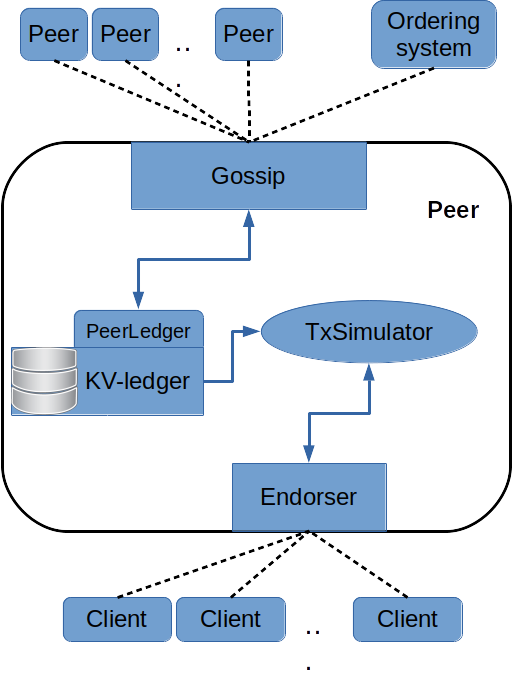
\includegraphics[width=0.5\textwidth]{figures/peer}
\end{center}
\caption{Relevant parts of a peer}
\label{fig:peer}
\end{figure}

Endorser subsystem is the one exposed to clients on the peer's side and it implements the Endorser gRPC service with a single call named ProcessProposal.
\begin{lstlisting}
rpc ProcessProposal(SignedProposal) returns (ProposalResponse) {}
\end{lstlisting}
SignedProposal is a structure sent by a client at the beginning of a transaction's lifecycle.

The Endorser subsystem executes the proposal, produces a read-write set as a result of the execution and creates a ProposalResponse which is used as an endorsement of the proposal by the client.  This subsystem has no direct access to the ledger. Access is provided indirectly through a transaction simulator (TxSimulator) produced by an endorser Support interface.

The Gossip subsystem handles all communications between all nodes of the network: peers and orderers alike. It is a big and intricate subsystem in and of itself and consists of many moving parts. However, for the purposes of the project, it is enough to know that Gossip handles block distribution and has capabilities to commit a block to the ledger.

KV-ledger subsystem implements PeerLedger interface and handles all the steps of committing a block to the ledger, described in \ref{sec:flow}. It is at this stage when each transaction goes through MVCC validation when versions of keys from read set are compared with versions from the ledger for consistency

It is important to note, that the Gossip service is a singleton and it is possible to access it globally from any part of the peer. However, the Endorser does not access it in its code. On the contrary, there is an instance of KV-ledger subsystem for each ledger hosted on the peer and it's not accessible to write to from the Endorser.
